\scanpage{18}
cette dernière, si $\operatorname{card}J=\operatorname{card}I-1=n-1$, on verra (par \unsure{rècurrence|récurrence}) que le cardinal de l'ens des classes est $(n-1)+1=n$.

Ceci posé, on voit d'abord que $E_i$ est dans
% G01: full-scan origin (820,465), x right/y down; manual geometry.
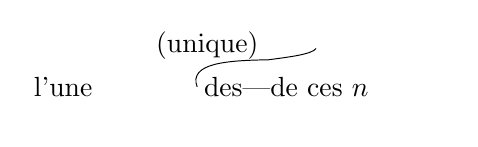
\begin{tikzpicture}[x=.08mm,y=-.08mm,baseline=(g01base)]
\path[use as bounding box] (0,0) rectangle (670,145);
\coordinate (g01base) at (0,115);
\begin{scope}[shift={(-820,-465)}]
\node[anchor=base west,inner sep=0pt,outer sep=0pt] at (830,574) {l'une};
\node[anchor=base west,inner sep=0pt,outer sep=0pt] at (1024,505) {\inserted{(unique)}};
\node[anchor=base west,inner sep=0pt,outer sep=0pt] at (1100,574) {\unsure{des|de} ces $n$};
\draw[line width=.35pt] (1089,559) .. controls (1075,521) and (1137,517) .. (1202,516) .. controls (1240,511) and (1271,507) .. (1278,498);
\end{scope}
\end{tikzpicture}
classes, qui sont des ouverts. Soit $U_{J,i}$ la classe (ou ``\unsure{composante|composant}'') qui contient $E_i$, et considérons les deux composantes $\Sigma_i^+,\Sigma_i^-$ de $X\setminus E_i$.

% G02: complete lemma group. Full-scan origin (244,1145).
% The underline and the left rule each occur once. The left rule begins
% below the first textual line; its observed endpoints are preserved.
\figure{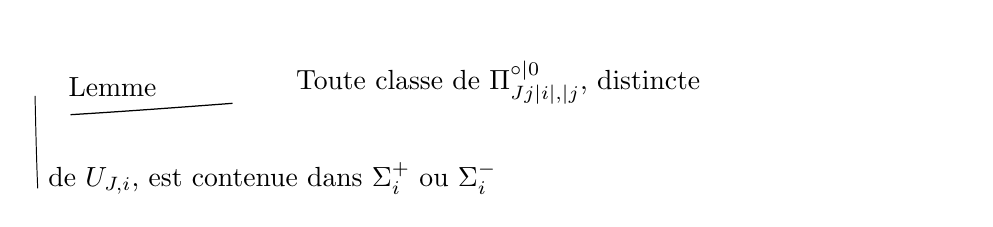
\begin{tikzpicture}[x=.085mm,y=-.085mm,baseline=(g02base)]
\path[use as bounding box] (0,0) rectangle (1400,255);
\coordinate (g02base) at (0,238);
\begin{scope}[shift={(-244,-1145)}]
\node[anchor=base west,inner sep=0pt,outer sep=0pt] at (305,1248) {\rlap{Lemme}\phantom{\uline{Lemme}}};
\node[anchor=base west,inner sep=0pt,outer sep=0pt] at (645,1238) {Toute classe de $\Pi_{J\unsure{\deleted{j}|\deleted{i}|\deleted{,}|j}}^{\unsure{\circ|0}}$, distincte};
\node[anchor=base west,inner sep=0pt,outer sep=0pt] at (275,1382) {de $U_{J,i}$, est contenue dans $\Sigma_i^+$ ou $\Sigma_i^-$};
\draw[line width=.45pt] (308,1275) .. controls (390,1270) and (471,1264) .. (550,1258);
\draw[line width=.35pt] (255,1247) .. controls (256,1290) and (257,1340) .. (259,1385);
\end{scope}
\end{tikzpicture}}

C'est presque une tautologie : Dire
% G03: qu'une/la/classe group, full-scan origin (235,1480), fixed 310 by 125 rectangle.
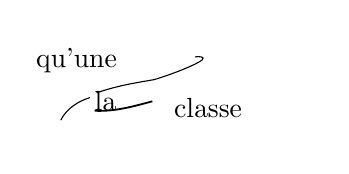
\begin{tikzpicture}[x=.012cm,y=-.012cm,baseline=(g03base)]
\path[use as bounding box] (0,0) rectangle (310,125);
\coordinate (g03base) at (0,91);
\begin{scope}[shift={(-235,-1480)}]
\node[anchor=base west,inner sep=0pt,outer sep=0pt] at (244,1522) {\inserted{qu'une}};
\node[anchor=base west,inner sep=0pt,outer sep=0pt] at (306,1568) {\rlap{la}\phantom{\deleted{la}}};
\node[anchor=base west,inner sep=0pt,outer sep=0pt] at (390,1575) {classe};
% G03a/b: observed interrupted insertion guide; the q descender belongs to qu'une.
\draw[line width=.4pt] (270,1578) .. controls (276,1566) and (288,1558) .. (301,1554);
\draw[line width=.4pt] (308,1549) .. controls (331,1541) and (352,1538) .. (369,1535) .. controls (389,1529) and (414,1519) .. (420,1514) .. controls (423,1511) and (417,1510) .. (412,1511);
% G03c: the actual lower cancellation stroke, without an additional generic rule.
\draw[line width=.65pt] (306,1568) .. controls (328,1569) and (348,1563) .. (367,1558);
\end{scope}
\end{tikzpicture}
% G04: donnée / inserted name / ne group. Full-scan origin (530,1445), fixed 525 by 160.
\begin{tikzpicture}[x=.010cm,y=-.010cm,baseline=(g04base)]
\path[use as bounding box] (0,0) rectangle (525,160);
\coordinate (g04base) at (0,111);
\begin{scope}[shift={(-530,-1445)}]
\node[anchor=base west,inner sep=0pt,outer sep=0pt] at (560,1556) {donnée};
\node[anchor=base west,inner sep=0pt,outer sep=0pt] at (797,1548) {ne};
\node[anchor=base west,inner sep=0pt,outer sep=0pt] at (737,1507) {\inserted{$U_{\unsure{\alpha|x}}$\quad de $\Pi_J^\circ$}};
% G04a: complete guide; no separate cancelled un is supplied.
\draw[line width=.4pt] (761,1554) .. controls (762,1540) and (791,1528) .. (811,1516) .. controls (853,1528) and (876,1534) .. (908,1521) .. controls (957,1511) and (1006,1500) .. (1012,1487);
% G04b: one locally qualified comma-like hook at the guide junction.
% Nested local origin (806,1504), baseline (0,0), base-west placement and zero separation.
% Its role as comma or guide return is unsettled; no second printed comma is added.
\node[anchor=base west,inner sep=0pt,outer sep=0pt] at (806,1504) {\unsure{\begin{tikzpicture}[x=.010cm,y=-.010cm,baseline=(g04hookbase)]
\path[use as bounding box] (0,0) rectangle (15,17);
\coordinate (g04hookbase) at (0,0);
\draw[line width=.45pt] (0,4) .. controls (9,0) and (15,6) .. (6,13);
\end{tikzpicture}}};
\end{scope}
\end{tikzpicture}
contient pas $\deleted{\Sigma}$\begin{tikzpicture}[x=.08mm,y=-.08mm,baseline=(g04base)]
% G04: corrected E_i and the separate upper stroke. Outer origin
% (1308,1480); inner overmark origin (1324,1492), baseline y=12.
% Closure-bar/remnant role is unresolved; the visible stroke is retained
% once, including its short returning right end, under local unsure.
\path[use as bounding box] (0,0) rectangle (85,85);
\coordinate (g04base) at (0,67);
\node[anchor=base west,inner sep=0pt,outer sep=0pt] at (0,67) {$E_i$};
\node[anchor=base west,inner sep=0pt,outer sep=0pt] at (16,24) {\unsure{\begin{tikzpicture}[x=.08mm,y=-.08mm,baseline=(g04markbase)]
\path[use as bounding box] (0,0) rectangle (55,12);
\coordinate (g04markbase) at (0,12);
\draw[line width=.45pt] (0,6) .. controls (17,5) and (34,6) .. (47,6) -- (31,10) -- (43,6);
\end{tikzpicture}}};
\end{tikzpicture}
i.e. est $\ne U_{J,i}$, signifie que il existe un $j\in J$ tel que le $\Sigma_j^+\in\pi_0(X\setminus\deleted{\Sigma}E_{\unsure{j|J}})$
% G05: source origin (1405,1720); uncertain word, single literal cancellation, two detached points.
\begin{tikzpicture}[x=.01cm,y=-.01cm,baseline={(0,50)}]
\path[use as bounding box] (0,0) rectangle (190,80);
\node[anchor=base west,inner sep=0,outer sep=0] at (0,50) {\rlap{\unsure{choisi|choisie}}\phantom{\deleted{\unsure{choisi|choisie}}}};
% G05.P1: cancellation run through the word.
\draw[line width=.65pt] (7,39) .. controls (55,40) and (109,41) .. (160,43);
% G05.P2-P3: detached points at fixed local origin (165,32); no character or role supplied.
\node[anchor=base west,inner sep=0,outer sep=0] at (165,32) {\unsure{\begin{tikzpicture}[x=.01cm,y=-.01cm,baseline=0pt]
\path[use as bounding box] (0,-8) rectangle (13,8);
\fill (2,2) ellipse [x radius=1,y radius=1.4];
\fill (8,-5) ellipse [x radius=.9,y radius=1.2];
\end{tikzpicture}}};
\end{tikzpicture}
``\unsure{composant|composante}'' de cette classe \deleted{est} est l'\unsure{é|e}l\unsure{ê|é}ment du $\pi_0$ qui ne contient pas $E_i$; il est donc contenu dans l'un des
% G06: whole éléments / (soit Sigma) / de / pi_0 group, origin (245,2135), fixed 795 by 155.
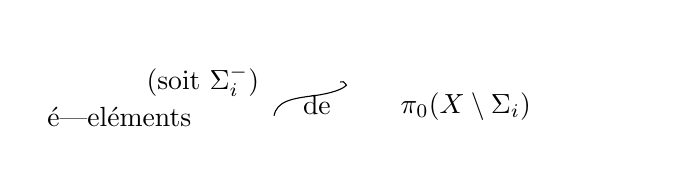
\begin{tikzpicture}[x=.010cm,y=-.010cm,baseline=(g06base)]
\path[use as bounding box] (0,0) rectangle (795,155);
\coordinate (g06base) at (0,125);
\begin{scope}[shift={(-245,-2135)}]
\node[anchor=base west,inner sep=0pt,outer sep=0pt] at (270,2260) {\unsure{é|e}léments};
\node[anchor=base west,inner sep=0pt,outer sep=0pt] at (396,2213) {\inserted{(soit $\Sigma_i^-$)}};
\node[anchor=base west,inner sep=0pt,outer sep=0pt] at (595,2245) {de};
\node[anchor=base west,inner sep=0pt,outer sep=0pt] at (719,2244) {$\pi_0(X\setminus\Sigma_i)$};
% G06a: guide crossing the ascender of de, with its full right hook.
\draw[line width=.4pt] (558,2247) .. controls (562,2228) and (580,2225) .. (612,2221) .. controls (632,2218) and (646,2213) .. (650,2208) .. controls (647,2204) and (645,2202) .. (642,2204);
\end{scope}
\end{tikzpicture}, d'après l'étude du
% G07: cas / cancelled deux / raised card I=2, origin (245,2240), fixed 370 by 123.
\begin{tikzpicture}[x=.012cm,y=-.012cm,baseline=(g07base)]
\path[use as bounding box] (0,0) rectangle (370,123);
\coordinate (g07base) at (0,85);
\begin{scope}[shift={(-245,-2240)}]
\node[anchor=base west,inner sep=0pt,outer sep=0pt] at (275,2325) {cas};
\node[anchor=base west,inner sep=0pt,outer sep=0pt] at (400,2321) {\rlap{\unsure{deux}}\phantom{\deleted{\unsure{deux}}}};
\node[anchor=base west,inner sep=0pt,outer sep=0pt] at (386,2302) {\inserted{$\operatorname{card}I=2$}};
% G07a: complete long cancellation rule, kept once.
\draw[line width=.65pt] (399,2320) .. controls (438,2313) and (483,2317) .. (515,2314) .. controls (531,2312) and (546,2311) .. (555,2312);
% G07b: supported lower hook below the I/= region; its guide/letter role remains unsettled.
% Nested origin (510,2290), baseline (0,0), base-west placement and zero separation.
\node[anchor=base west,inner sep=0pt,outer sep=0pt] at (510,2290) {\unsure{\begin{tikzpicture}[x=.012cm,y=-.012cm,baseline=(g07hookbase)]
\path[use as bounding box] (0,0) rectangle (12,27);
\coordinate (g07hookbase) at (0,0);
\draw[line width=.5pt] (4,4) .. controls (10,10) and (8,18) .. (1,24);
\end{tikzpicture}}};
\end{scope}
\end{tikzpicture},
\deleted{\unsure{cela|OK|et}} \unsure{â|à} fortiori $U_\alpha\subset\Sigma_i^-$,
% G08: source origin (1440,2250). OK's rising stroke has unresolved joining/cancellation state.
\begin{tikzpicture}[x=.01cm,y=-.01cm,baseline={(0,55)}]
\path[use as bounding box] (0,0) rectangle (210,95);
\node[anchor=base west,inner sep=0,outer sep=0] at (11,55) {\unsure{\begin{tikzpicture}[x=.01cm,y=-.01cm,baseline=0pt]
\path[use as bounding box] (0,-45) rectangle (85,8);
\node[anchor=base west,inner sep=0,outer sep=0] at (0,0) {\rlap{OK}\phantom{\deleted{OK}}};
% G08.P1: the visible rising crossing/joining stroke, drawn only here.
\draw[line width=.35pt] (0,-15) .. controls (24,-21) and (51,-32) .. (73,-40);
\end{tikzpicture}}};
\node[anchor=base west,inner sep=0,outer sep=0] at (127,61) {.};
% G08.P2: faint detached spot; shape, hand, surface origin and role remain qualified.
\node[anchor=base west,inner sep=0,outer sep=0] at (192,42) {\unsure{\begin{tikzpicture}[x=.01cm,y=-.01cm,baseline=0pt]
\path[use as bounding box] (0,0) rectangle (6,6);
\fill[gray] (2,2) ellipse [x radius=1.1,y radius=1.6];
\end{tikzpicture}}};
\end{tikzpicture}
% archive sheet number: 17
